%
% ACMD 2026 full paper (10-page limit, single-column A4, acmd2026_fullpaper.cls).
% Cut/reformatted from the extended IEEEtran draft (paper.tex, tag journal-draft),
% which remains the seed for the JSME Mechanical Engineering Journal special issue.
%
\documentclass{acmd2026_fullpaper}
\graphicspath{{paper_figures/}}

\begin{document}

%------------------------------------------------------------ title
\begin{center}
  \fontsize{12}{16}{\bf
    Terrain-Aware, Latency-Robust Control for Off-Road Autonomy \\
    and Teleoperation on Deformable Terrain}
\end{center}

%------------------------------------------------------------ authors
\begin{center}
\normalsize{\bf{
  \underline{Kyle Sha}, Zhenhao Zhou, Radu Serban, Dan Negrut}}
\end{center}

%------------------------------------------------------------ affiliation
\begin{center}
  \begin{tabular}{c}
    Department of Mechanical Engineering \\
    University of Wisconsin--Madison \\
    1513 University Ave., Madison, WI 53706, USA \\
    \{kasha2, zzhou292, serban, negrut\}@wisc.edu \\
  \end{tabular}
\end{center}

%------------------------------------------------------------ abstract
\section*{ABSTRACT}
We present a modular, latency-aware framework for shared and autonomous control
of ground vehicles on deformable Soil Contact Model (SCM) terrain, in which
terrain adaptation, command screening, latency compensation, and advisory
warning run on one plant and message stream so their cross-layer effects can be
measured together. The framework exposes six extension points: command source,
safety filter, collision warning, tire model, terrain estimator, and latency
profile. A differentiable neural tire model is embedded in an \emph{acados}
nonlinear MPC (NMPC); an online force/proprioceptive estimator recovers the
Bekker sinkage exponent and re-conditions the tire model from inertial and
wheel-speed signals; and an asymmetric throttle disturbance observer removes the
residual soft-soil speed deficit. Obstacle avoidance is a two-layer stack:
in-horizon NMPC barriers backed by a swappable downstream safety filter whose
default is an intent-preserving, minimum-deviation disturbance-observer control
barrier function (DOB-CBF) suited to teleoperation. A terrain- and latency-aware
forward collision warning reuses the same tire model for a soil-conditioned
braking budget and advises the operator without overriding commands. The plant
is Chrono::Vehicle within Chrono::HIL, driven by a synthetic 5G latency trace on
the command and camera channels. Across repeatable simulation experiments the
neural stack cuts median RMS crosstrack error by 39--41\% versus SCM-calibrated
Pacejka and TMeasy baselines, concentrated in off-nominal cells; the fused
estimator tracks the sinkage exponent to 3.8\% median error, the best of four
backends; the DOB-CBF filter cuts collisions by 88\% under the 5G profile, with
a deterministic counterfactual attributing 36 of 45 averted collisions to it;
and the collision warning reproduces Chrono brake-stop distances to 0.17~m. An
integrated mission runs all layers together collision-free across a
clay-to-sand transition.

%------------------------------------------------------------
\section{INTRODUCTION}
Off-road teleoperation contends with two compounding uncertainties: time-varying
soil mechanics that rigid-terrain tire models cannot capture without
per-deployment recalibration~\cite{Dallas21,Bekker69}, and time-varying network
latency that destabilises naive shared-control arbitration~\cite{Choi23,Zhang25}.
These are usually addressed in isolation: terrain-adaptive planning assumes
nominal communication, while delay-compensated safety assumes rigid-terrain
dynamics. This paper integrates the two into a single closed-loop framework and
reports paired simulation studies that isolate the main cross-layer choices.

The framework spans four coupled layers around one deformable-terrain plant:
(i) a terrain-aware NMPC built on a differentiable neural tire model; (ii) an
online terrain estimator that re-conditions that model from onboard sensors;
(iii) a two-layer obstacle-avoidance stack (in-horizon barriers plus a swappable
downstream safety filter) for autonomous and teleoperated commands; and (iv) a
terrain- and latency-aware forward collision warning that reuses the same tire
model for an advisory channel when an override-style filter is undesirable. All
four share one Chrono::Vehicle plant inside Chrono::HIL~\cite{Zhou23}, one
message stream, and one benchmarking harness, so the main comparisons run on one
matrix. The contribution is the \emph{integration}: evaluating these layers
head-to-head on shared infrastructure exposes cross-layer interactions that
isolated studies cannot, such as the safety filter and the collision warning
both re-using the controller's tire model for their traction and braking
budgets. This paper summarises the headline results; an extended version reports
the full ablation set.

%------------------------------------------------------------
\section{FRAMEWORK}
The runtime is organised around six extension points (Fig.~\ref{fig:arch},
Table~\ref{tab:swap}), each declared as a typed interface with a registry.
Chrono::Vehicle simulates an HMMWV on an SCM~\cite{Krenn09} patch within
Chrono::HIL. The simulation and controller run as separate processes and
exchange messages over ROS~2 topics through Chrono::ROS, so any node that
subscribes to the vehicle state and publishes a control command can replace the
NMPC without touching the simulator; this is how the tire-model variants are
evaluated. Human teleoperation reduces to the same normalised steering,
throttle, and brake channels before actuation, so the safety layer screens
autonomous and human commands behind one contract. The controller-to-simulation
message carries the live terrain estimate as optional fields, so the sim-side
safety filter re-conditions itself without a separate channel.

\begin{figure}[t]
  \begin{center}
    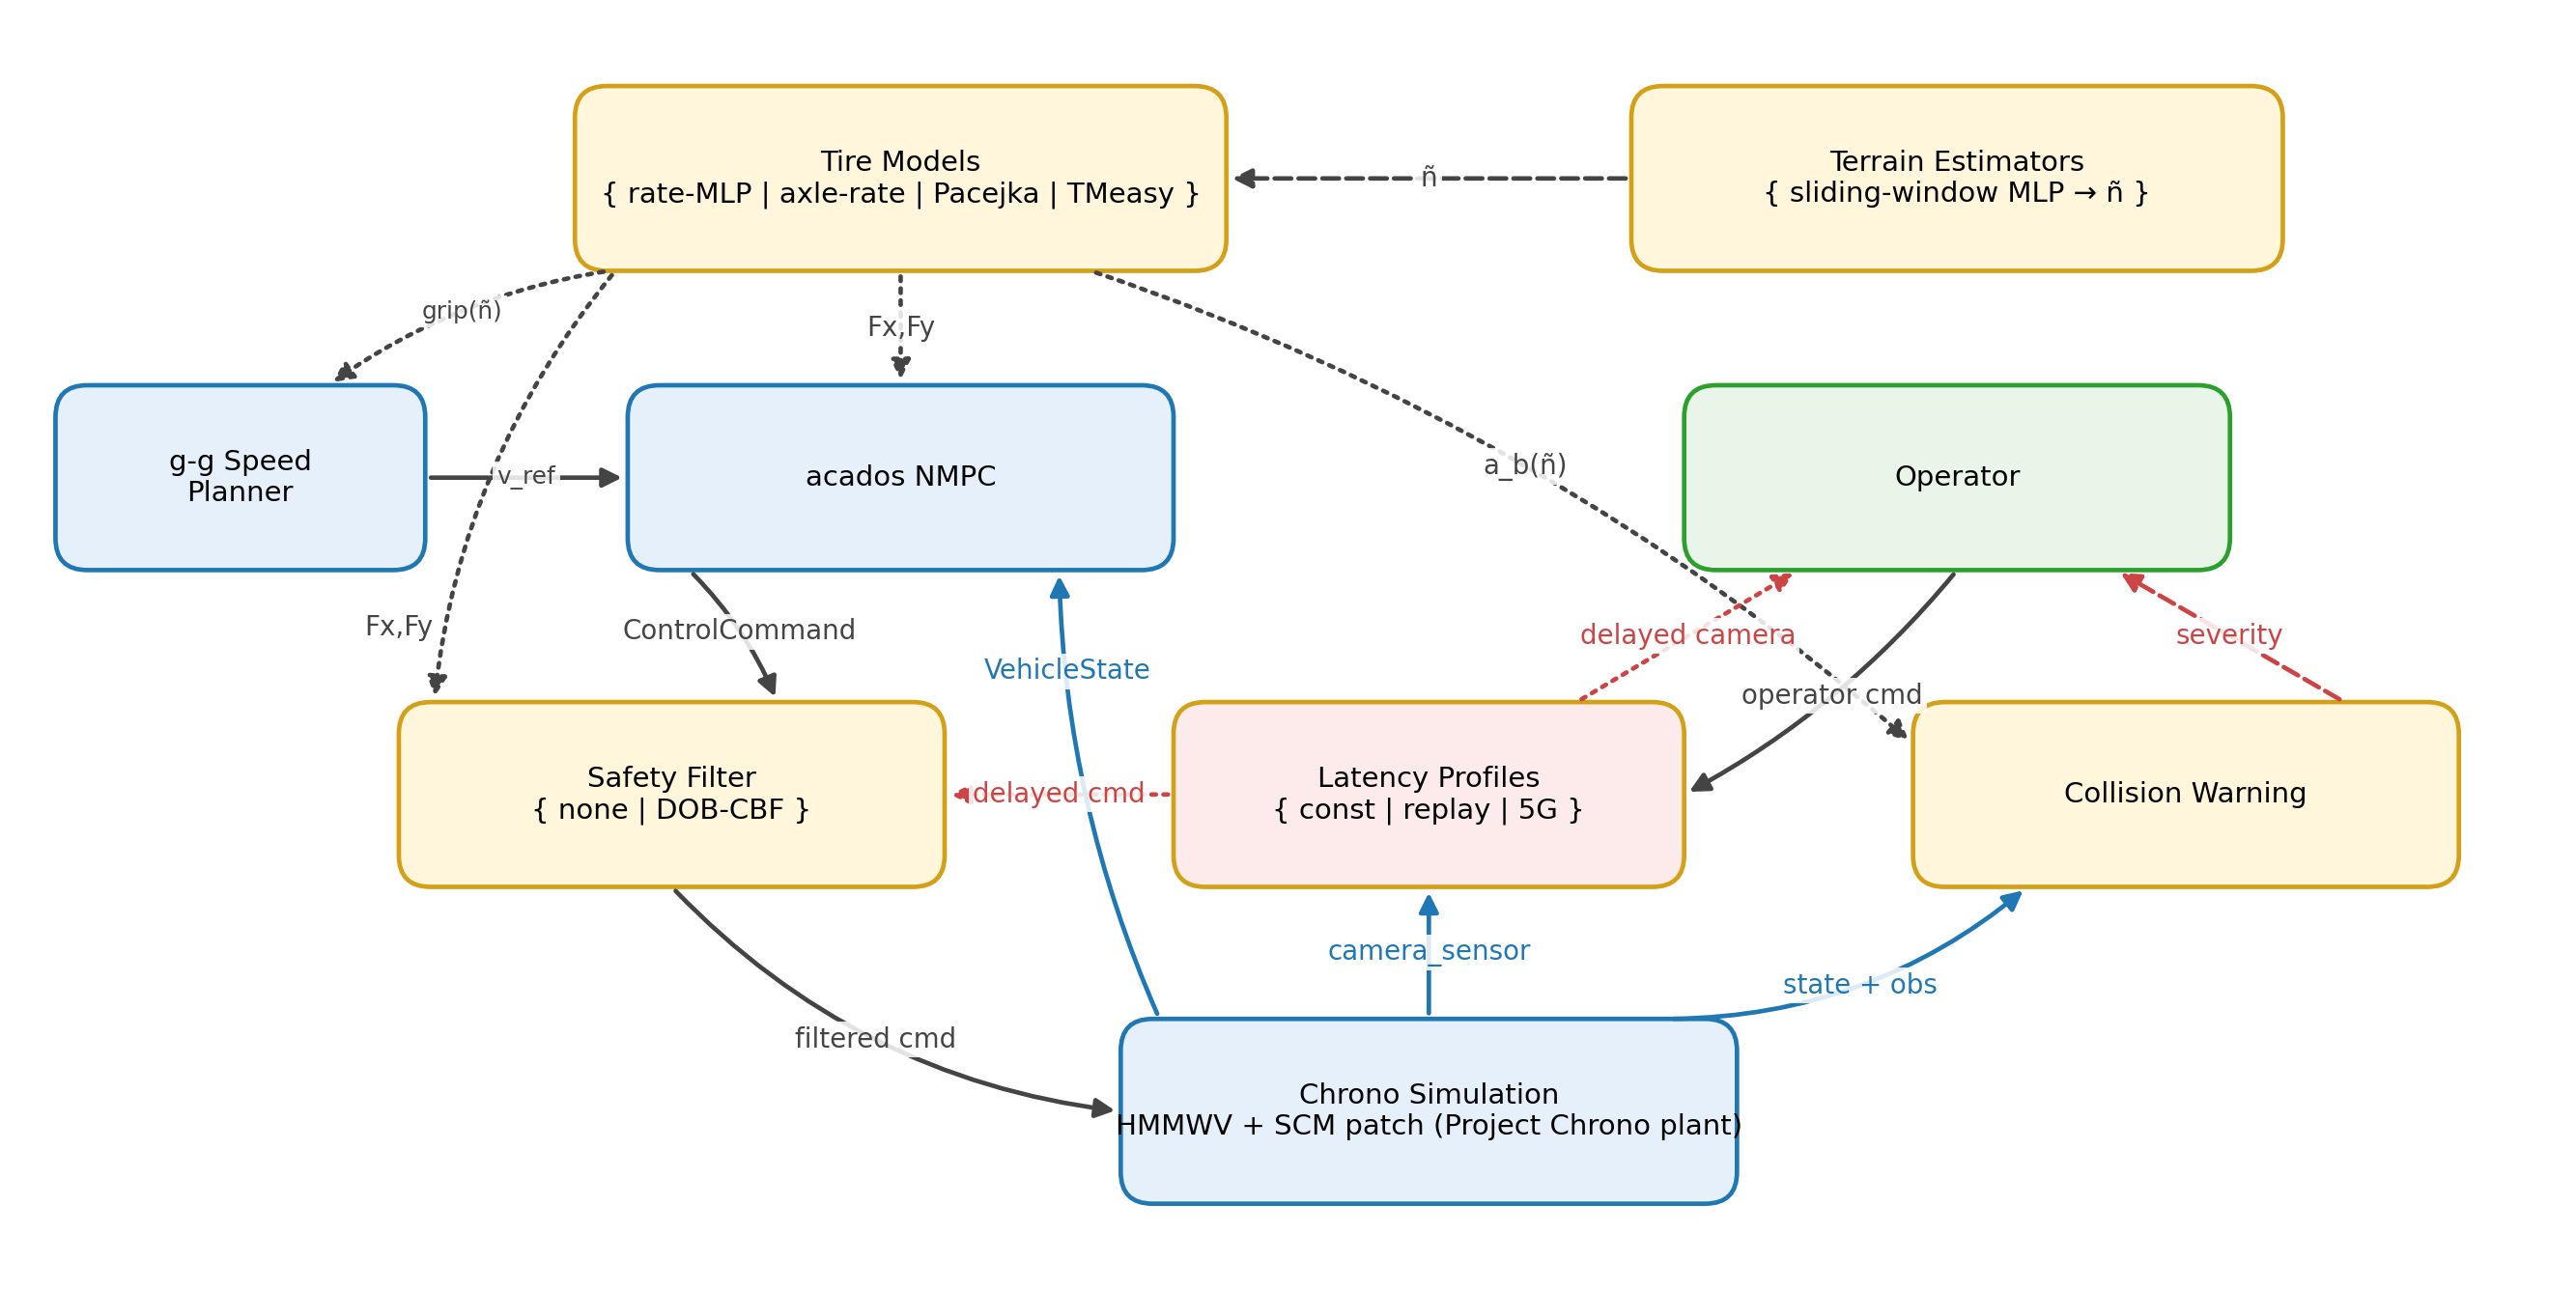
\includegraphics[width=0.98\textwidth]{sys_arch.png}
    \figcaption{Shared-control framework. Yellow nodes are in-process extension
      points; blue/green nodes are process-boundary or operator endpoints. Solid
      arrows are runtime data flow; dashed arrows are latency-affected operator
      paths; dotted arrows are tire-model queries.}
    \label{fig:arch}
  \end{center}
\end{figure}

\begin{table}[t]
  \begin{center}
    \tabcaption{The six extension points of the framework.}
    \vspace{1mm}
    \small
    \begin{tabular}{lll}
      \toprule
      \textbf{Role} & \textbf{Interface} & \textbf{Variants}\\
      \midrule
      Command source    & \texttt{next\_command} & NMPC, G29, WASD\\
      Safety filter     & \texttt{filter}        & DOB-CBF; none\\
      Collision warning & \texttt{evaluate}      & TTC\\
      Tire-force model  & \texttt{predict}       & rate-MLP, Pacejka, TMeasy\\
      Terrain estimator & \texttt{estimate}      & Fused-UKF, window-MLP, Bekker-UKF\\
      Latency profile   & \texttt{delay}         & constant, replay, learned 5G\\
      \bottomrule
    \end{tabular}
    \label{tab:swap}
  \end{center}
\end{table}

%------------------------------------------------------------
\section{TERRAIN-AWARE CONTROL AND TIRE SURROGATE}
A multilayer perceptron maps the tire operating point
$(\kappa,\alpha,F_z,u)$, steering rate, and the six Bekker--Mohr soil parameters
to longitudinal and lateral forces $(F_x,F_y)$. Extending the static map of
Dallas et al.~\cite{Dallas21}, a rate-augmented variant adds the steering rate
as an input so the model represents the transient force during fast steering.
The surrogate is trained on controlled single-tire SCM sweeps --- one tire on a
virtual test rig, stepped over a grid of operating points with the exact SCM
force logged at each (the reproducible protocol of~\cite{Dallas21}). Every
training label is therefore exact, no closed-loop feedback confounds the
supervision, and the data collection parallelises trivially. The trained model
exports as a CasADi expression through which the acados solver
auto-differentiates at every horizon stage.

Table~\ref{tab:tire} reports the static-terrain benchmark against Pacejka and
TMeasy baselines calibrated to the SCM plant's mean lateral friction
($\mu=0.42$). The neural surrogate cuts mean RMS crosstrack error by
$\approx$58\% versus both analytical baselines
($0.16$ vs.\ $0.38$~m), a gain concentrated in the off-nominal cells (dirt,
higher speed) where the fixed force laws lose grip (Fig.~\ref{fig:cte}); on
benign cells the models are comparable. The longitudinal channel carries a
terrain-dependent motion-resistance bias that the throttle disturbance observer
(\S\ref{sec:speed}) absorbs online rather than a tire-model deficit, and
conditioning the surrogate on the online terrain estimate (\S\ref{sec:est})
recovers near-oracle tracking with no prior terrain knowledge.

\begin{table}[t]
  \begin{center}
    \tabcaption{Static-terrain tire-model benchmark (mean $\pm$ std RMS
      crosstrack error; 405 runs per model over 3 terrains $\times$ 3 paths
      $\times$ 3 speeds $\times$ 3 bumpiness $\times$ 5 seeds). The rig neural
      surrogate attains the lowest error, $\approx$58\% below the SCM-calibrated
      analytical baselines.}
    \vspace{1mm}
    \small
    \begin{tabular}{lccc}
      \toprule
      \textbf{Tire model} & \textbf{RMS CTE (m)} & \textbf{Speed ratio} & \textbf{Solve (ms)}\\
      \midrule
      Pacejka             & $0.38 \pm 0.50$ & 0.67 & 3.9\\
      TMeasy              & $0.37 \pm 0.49$ & 0.66 & 4.0\\
      Rig NN rate-MLP     & $\mathbf{0.16 \pm 0.12}$ & 0.66 & 11.2\\
      \bottomrule
    \end{tabular}
    \label{tab:tire}
  \end{center}
\end{table}

\begin{figure}[t]
  \begin{center}
    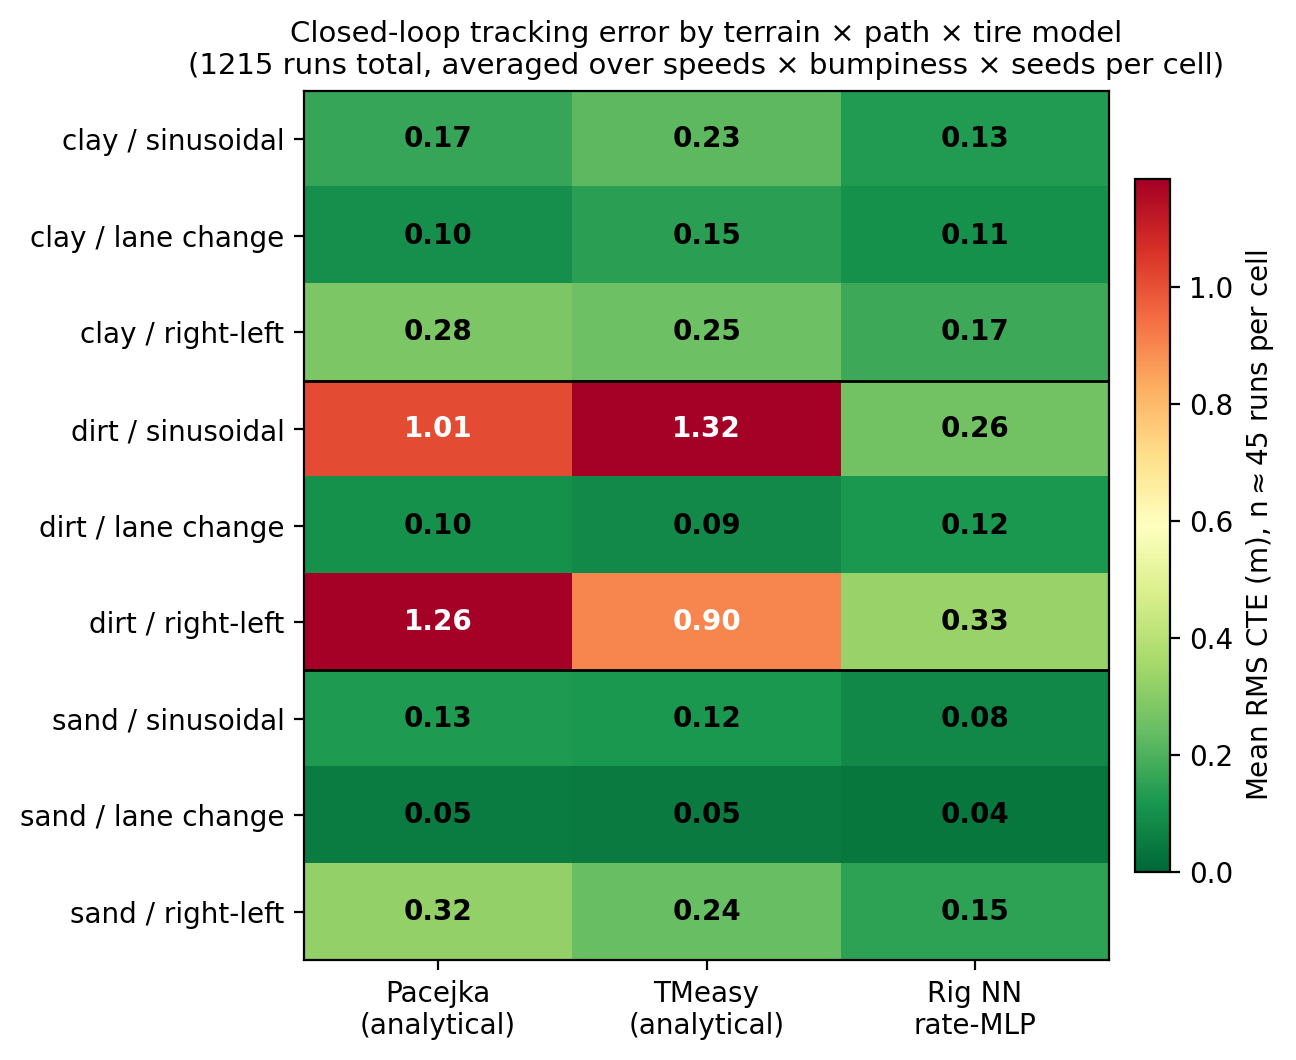
\includegraphics[width=0.85\textwidth]{cte_master_heatmap.png}
    \figcaption{Closed-loop RMS crosstrack error per (terrain, path) cell. The
      analytical baselines diverge on dirt (\,$\sim$1.0--1.2~m) where the
      curvature-limited reference meets off-nominal sinkage; the neural model
      suppresses those tails while matching the baselines on benign cells.}
    \label{fig:cte}
  \end{center}
\end{figure}

%------------------------------------------------------------
\section{ONLINE TERRAIN ESTIMATION}
\label{sec:est}
The deployed estimator is a state-augmented unscented Kalman filter (Fused-UKF)
that estimates the Bekker sinkage exponent $n$ jointly with the bicycle state
and fuses \emph{two} measurement channels: a whole-vehicle lateral-force
surrogate that predicts $(F_{y},M_{\mathrm{yaw}})$ from the bicycle state and
soil parameters, and a proprioceptive sliding-window MLP that regresses $n$ from
a 4\,s window of inertial and wheel-speed statistics together with a per-sample
uncertainty. The two are weighted purely by Kalman covariance, with no
hand-tuned gate. Only $n$ is identified online; the remaining five Bekker--Mohr
parameters are reconstructed from $\hat n$ along the clay--dirt--sand preset
manifold (the parameter-known setting).

The force channel alone is blind to firm-soil $n$ under gentle path tracking: at
small slip the lateral-force signal separating firm from soft soil
($\approx\!130$~N) sits below the lateral-accel noise floor ($\approx\!770$~N),
so a force-only filter cannot observe $n$ once closed-loop slip is small. The
proprioceptive channel reads vibration rather than slip-dependent force and
fills exactly this gap. Table~\ref{tab:est} and Fig.~\ref{fig:est} report a
head-to-head over 100 soils swept along the Bekker--Mohr manifold: the two
force-only backends saturate near $n\!\approx\!0.6$ on firm soils
(19--20\% median error), whereas the Fused-UKF tracks $n$ across the full range
at 3.8\% median error (94\% of soils within $\pm$20\%), the best of four
backends.

\begin{table}[t]
  \begin{center}
    \tabcaption{Closed-loop terrain-estimator head-to-head, 100 soils on the
      clay--dirt--sand manifold. Tail-window $|\Delta n|$ (absolute and
      relative).}
    \vspace{1mm}
    \small
    \begin{tabular}{lccc}
      \toprule
      \textbf{Estimator} & \textbf{median $|\Delta n|$} & \textbf{median \%err} & \textbf{within $\pm$20\%}\\
      \midrule
      Window-MLP  & 0.060 & 7.8\%  & 76\%\\
      Bekker-UKF  & 0.154 & 19.9\% & 50\%\\
      NN-UKF      & 0.146 & 19.1\% & 55\%\\
      \textbf{Fused-UKF} & \textbf{0.033} & \textbf{3.8\%} & \textbf{94\%}\\
      \bottomrule
    \end{tabular}
    \label{tab:est}
  \end{center}
\end{table}

\begin{figure}[t]
  \begin{center}
    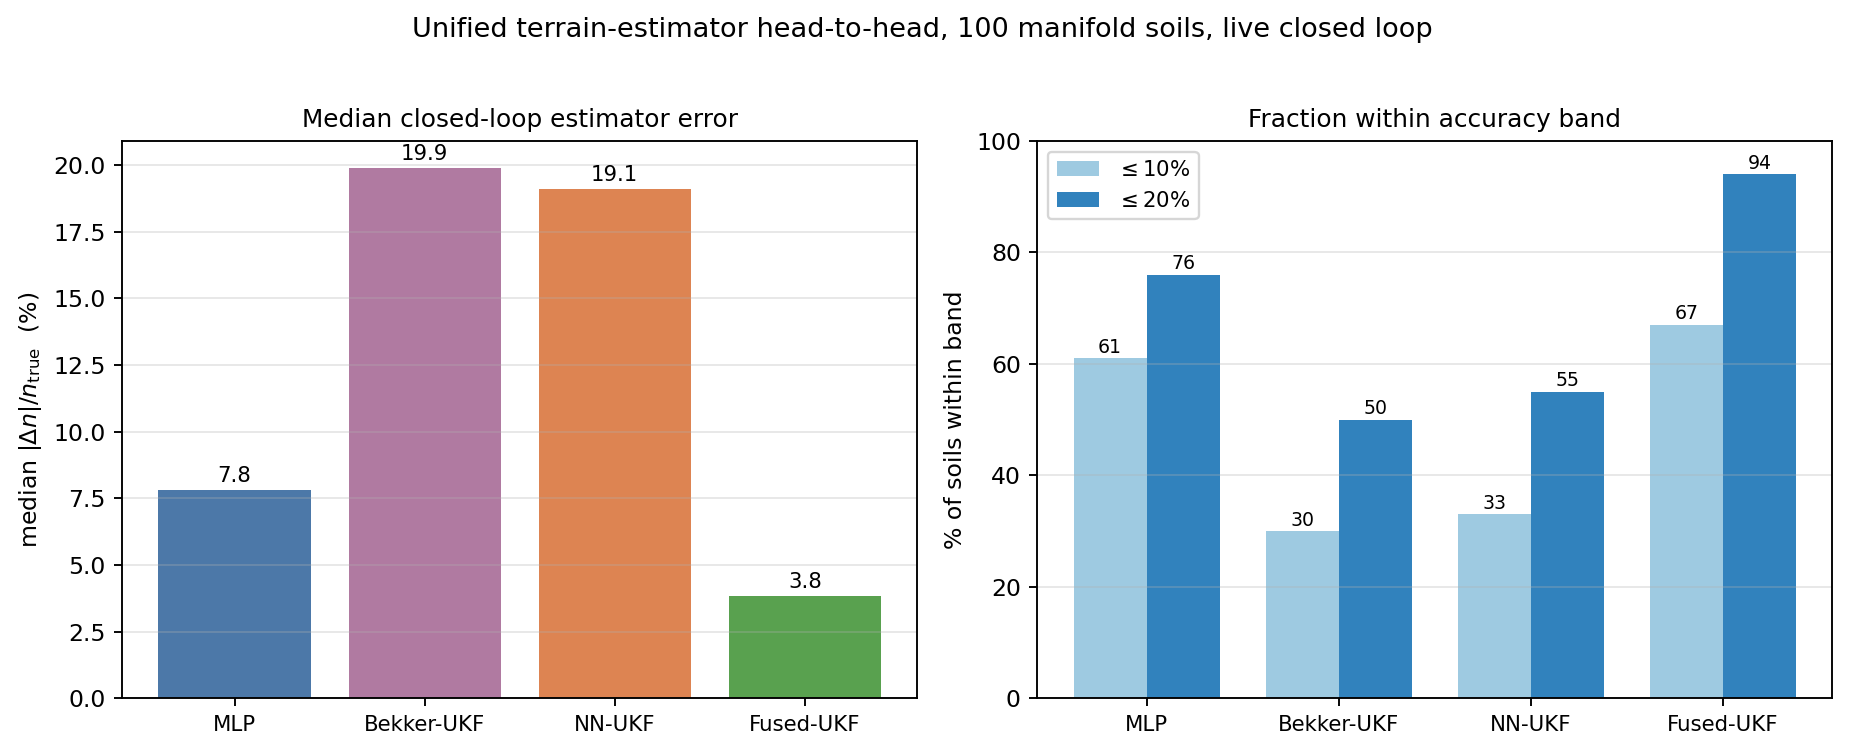
\includegraphics[width=0.98\textwidth]{estimator_overall.png}
    \figcaption{Pooled estimator comparison over the 100 manifold soils.
      \textbf{Left:} median relative error. \textbf{Right:} fraction within the
      $\pm$10\%/$\pm$20\% bands. The force-only UKFs trail because they cannot
      observe $n$ on firm soils in closed loop.}
    \label{fig:est}
  \end{center}
\end{figure}

A separate ablation isolates the estimator's deployable value directly. Holding
the controller's terrain prior at dirt regardless of the plant terrain gives a
wrong-prior baseline, compared on the same matrix against the matched-prior
oracle and the estimator-on variant (Table~\ref{tab:wrongprior}). On clay the
wrong dirt prior yields 1.53~m RMS crosstrack error; the estimator adapts from
the same dirt initialisation to 0.63~m, close to the matched-prior oracle
(0.49~m) --- closing $\approx$86\% of the prior-mismatch gap on the harder
terrain, with no prior terrain knowledge.

\begin{table}[t]
  \begin{center}
    \tabcaption{Wrong-prior ablation: RMS crosstrack error (m) with the
      controller's terrain prior fixed to dirt regardless of plant terrain, vs.\
      the matched-prior oracle and the estimator-on variant (60 runs).}
    \vspace{1mm}
    \small
    \begin{tabular}{lccc}
      \toprule
      \textbf{Variant} & \textbf{Clay} & \textbf{Sand} & \textbf{Mean}\\
      \midrule
      Matched static prior (oracle)   & 0.486 & 0.056 & 0.271\\
      Wrong (dirt) static prior        & 1.528 & 0.061 & 0.794\\
      Estimator-on (dirt $\to$ adapt)  & 0.632 & 0.059 & 0.346\\
      \bottomrule
    \end{tabular}
    \label{tab:wrongprior}
  \end{center}
\end{table}

%------------------------------------------------------------
\section{SPEED PLANNING AND DISTURBANCE OBSERVER}
\label{sec:speed}
A purely geometric curvature-limited speed reference is blind to the soil and
commands cornering speeds the available grip cannot support. We replace it with
a terrain-aware friction-circle (g--g) profile that queries the tire model at
the live $\hat n$ for the available lateral and tractive force and returns the
fastest reference that keeps the combined demand inside the circle. Against the
geometric reference this cuts mean RMS crosstrack error by 36\%
($0.136\!\to\!0.087$~m) for a 7\% reduction in mean speed, concentrated on the
soft-soil high-speed cells where crosstrack error falls 58--71\%.

On deformable soil the realised longitudinal acceleration is smaller than
commanded because of sinkage drag, producing a steady-state under-speed bias. An
asymmetric integral disturbance observer on the actuation map absorbs it,
accumulating during under-speed and bleeding slowly so it never adds an
over-speed bias. It raises achieved speed by $\approx$5\%
($0.61\!\to\!0.64$ of the g--g profile) at a $\sim$2\,mm tracking cost. The bias
is terrain-dependent and sign-varying (firm soil over-predicts speed, soft dirt
under-predicts), so an adaptive observer beats a fixed feedforward drag term.

\begin{figure}[t]
  \begin{center}
    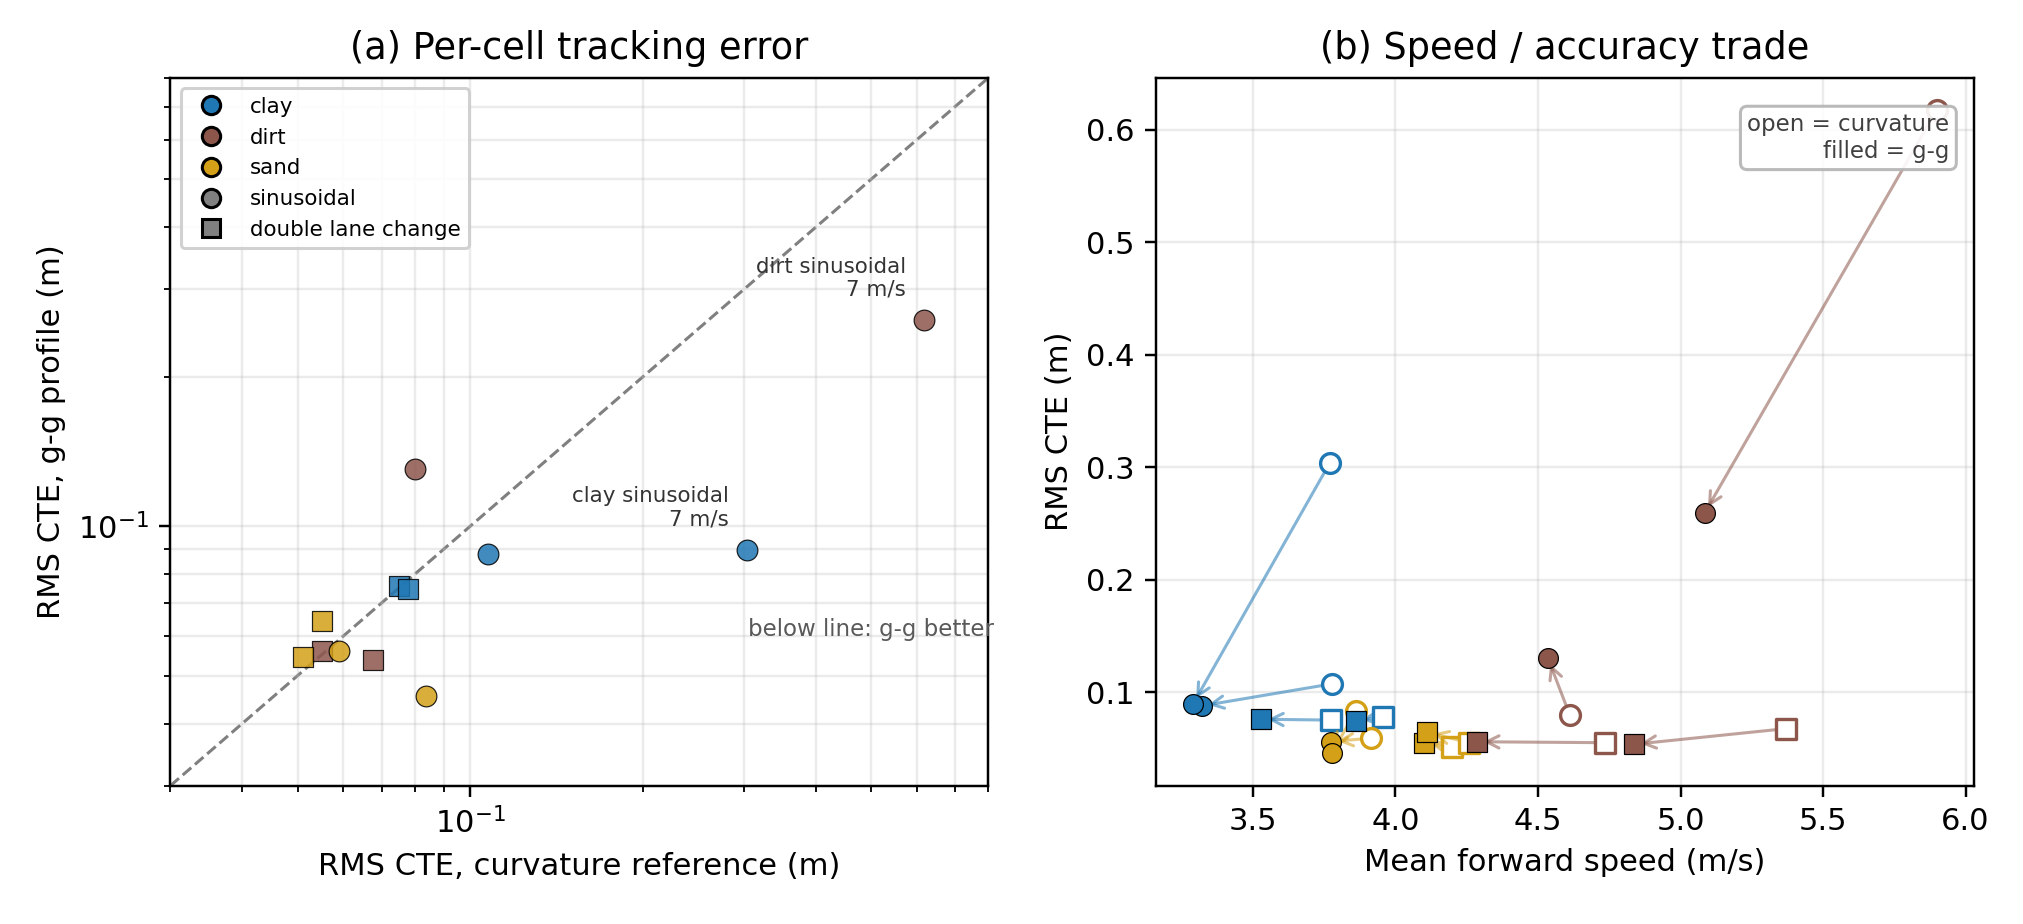
\includegraphics[width=0.98\textwidth]{speed_profile_gg.png}
    \figcaption{Terrain-aware g--g speed profile vs.\ the geometric curvature
      reference. \textbf{(a)} Per-cell RMS crosstrack error: the soft-soil
      high-speed cells drop to the trackable cluster while benign cells are
      unchanged. \textbf{(b)} Speed/accuracy trade: each cell trades a little
      mean speed for a large error reduction. Grip limits come live from the tire
      model at $\hat n$.}
    \label{fig:gg}
  \end{center}
\end{figure}

%------------------------------------------------------------
\section{OBSTACLE AVOIDANCE AND LATENCY ROBUSTNESS}
The planner adds smooth barriers to the NMPC cost for each known obstacle.
Downstream, a swappable safety filter screens the desired command; the default
DOB-CBF solves a single-step minimum-deviation quadratic program around the
incoming command~\cite{Ames19,Zhang25} with a disturbance-observer traction
budget and physical rate limits, the natural intent-preserving mechanism for
teleoperation. It carries obstacle-type awareness and a rear-approach guard, and
delay compensation that inflates its obstacle buffer by a delay-dependent
stopping distance.

Because a human operator cannot be driven consistently under latency, the
headline safety result is a deterministic \emph{counterfactual}: a fixed command
trace is replayed through the identical scenario with the filter off and on, so
every outcome difference is attributable to the filter. Over a population of
scripted worst-case ``drive-into-hazard'' commands across five dynamic-traffic
(convoy) scenarios and three command delays (45 cells), the unfiltered intent
collides in all 45; DOB-CBF prevents 36, cutting the collision rate from 100\%
to 20\% and turning a mean clearance of $-2.23$~m into $+2.25$~m at small command
deviation (Table~\ref{tab:safety}, Fig.~\ref{fig:cf}). The same machinery
replays recorded G29 human traces unchanged.

With the in-horizon barrier re-enabled the honest attribution is two-layer: the
barrier alone cuts collisions $\sim$5$\times$ (3.05$\to$0.57 per run), and adding
DOB-CBF drives them to 0.12 per run, a 96\% reduction over the blind baseline at
the lowest intervention rate of any configuration. Under the learned 5G profile
(a sequence model fit to a public uplink dataset~\cite{Choi23}, mapped to
per-channel delays), DOB-CBF cuts collisions by 88\% (2.74$\to$0.34 per run). A
paired blind-vs-aware ablation confirms the gain is the \emph{delay awareness},
not merely having a filter: the gap grows with delay, and by 0.5~s awareness
removes the residual collisions the delay-blind filter still suffers
(Fig.~\ref{fig:lat}).

\begin{figure}[t]
  \begin{center}
    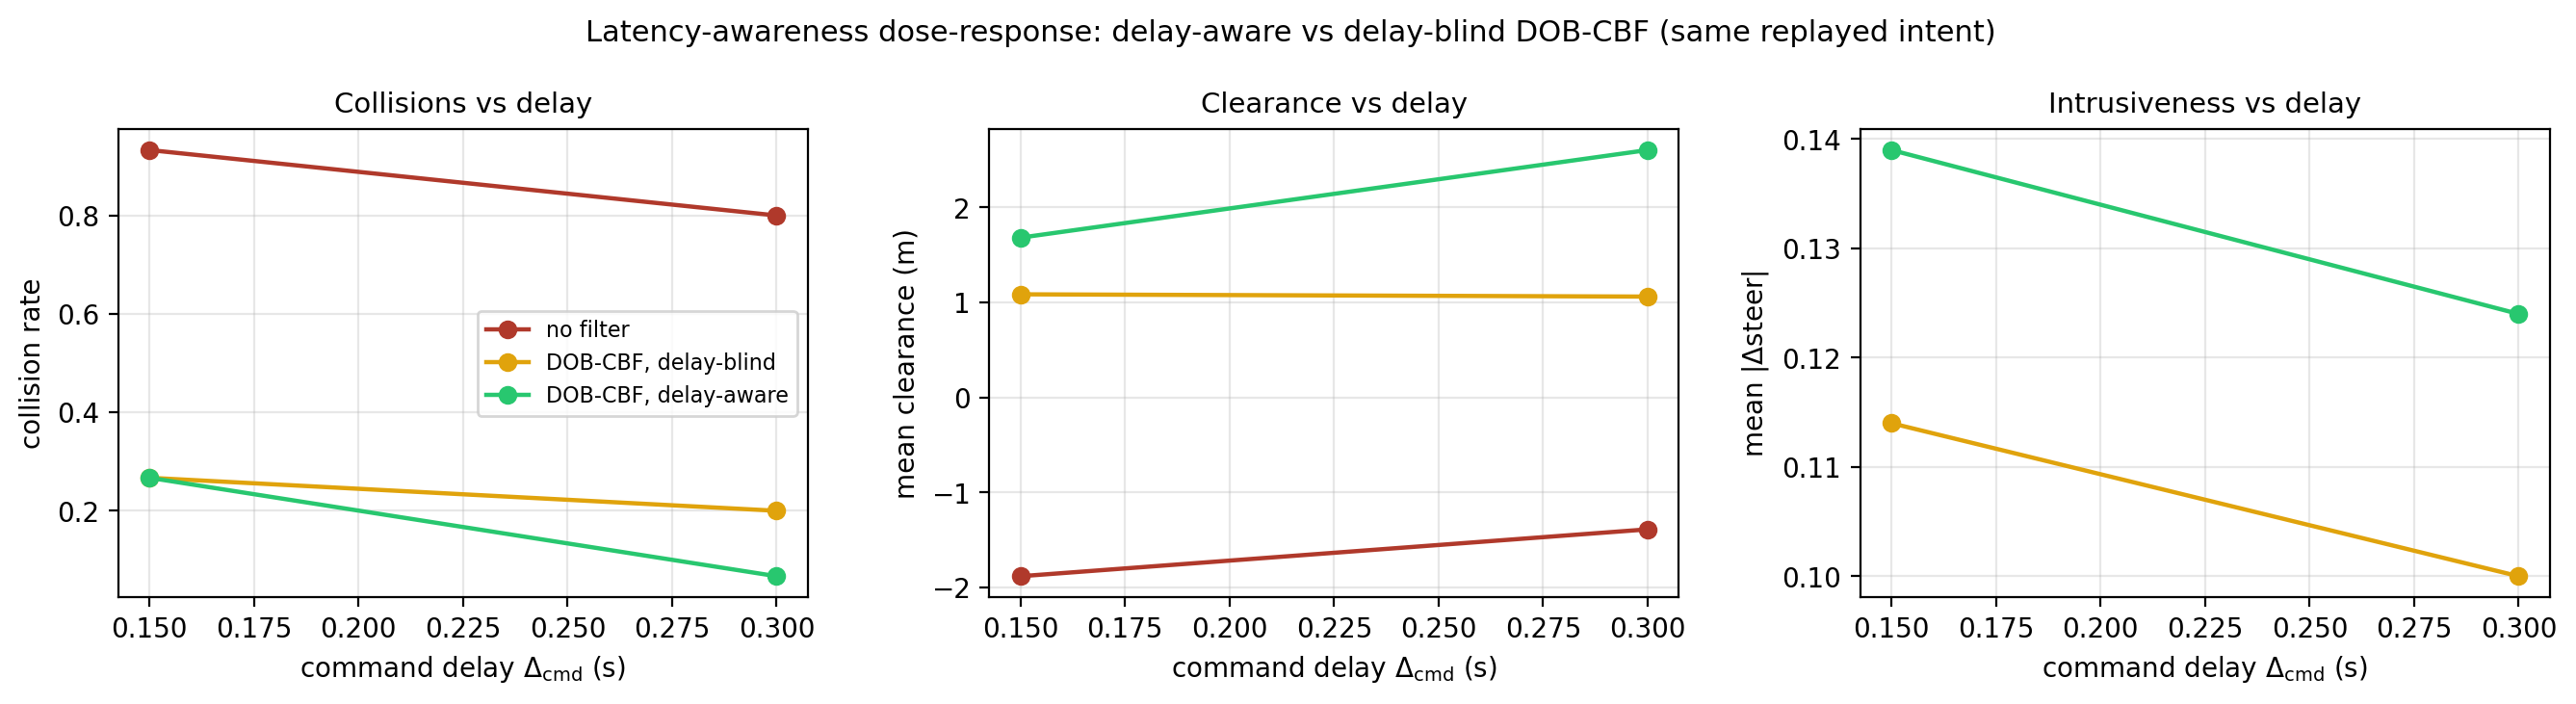
\includegraphics[width=0.80\textwidth]{latency_awareness_ablation.png}
    \figcaption{Latency-awareness dose-response: the same worst-case commands
      replayed with the DOB-CBF filter told the command delay (aware) or not
      (blind). At zero delay the two coincide; the gap grows with delay, and by
      0.5~s awareness removes the residual collisions at comparable
      intrusiveness.}
    \label{fig:lat}
  \end{center}
\end{figure}

\begin{table}[t]
  \begin{center}
    \tabcaption{Counterfactual convoy replay (45 cells per filter): scripted
      worst-case commands replayed filter-off vs.\ DOB-CBF.}
    \vspace{1mm}
    \small
    \begin{tabular}{lcccc}
      \toprule
      \textbf{Filter} & \textbf{Coll.\ rate} & \textbf{Prevented} & \textbf{Clearance (m)} & \textbf{$|\Delta\delta|$}\\
      \midrule
      None    & 1.00 (45/45) & ---   & $-2.23$ & ---\\
      DOB-CBF & 0.20 (9/45)  & 36/45 & $+2.25$ & 0.13\\
      \bottomrule
    \end{tabular}
    \label{tab:safety}
  \end{center}
\end{table}

\begin{figure}[t]
  \begin{center}
    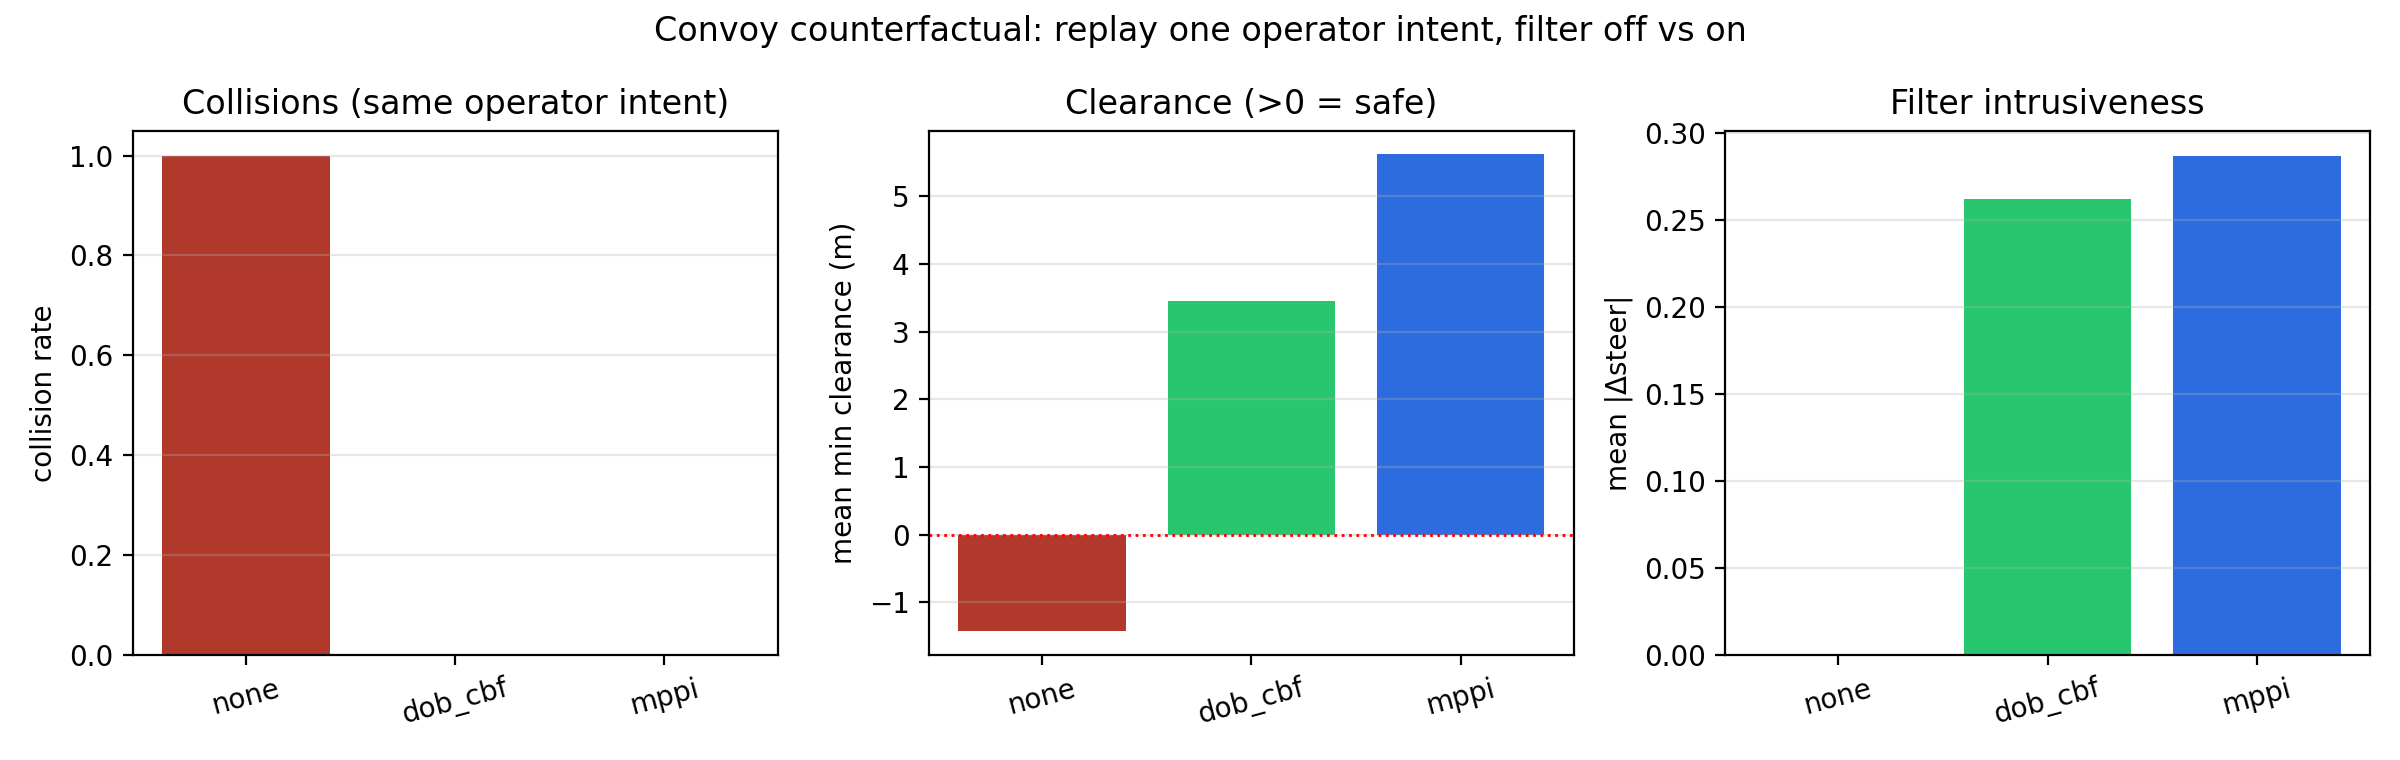
\includegraphics[width=0.98\textwidth]{convoy_counterfactual.png}
    \figcaption{Counterfactual replay on recorded human G29 drives (convoy
      scenarios under good/congested 5G latency), operator vs.\ DOB-CBF. The
      filter averts the forward-collision cases and lifts the median minimum
      clearance, without fighting a capable driver.}
    \label{fig:cf}
  \end{center}
\end{figure}

\begin{table}[t]
  \begin{center}
    \tabcaption{Planner-aware vs.\ planner-blind safety sweep (1620 runs). The
      two-layer stack (barrier $+$ DOB-CBF) drives collisions to 0.12/run while
      reducing intervention and command deviation.}
    \vspace{1mm}
    \small
    \begin{tabular}{lccc}
      \toprule
      \textbf{Variant} & \textbf{Coll./run} & \textbf{Clearance (m)} & \textbf{Interv.\ (\%)}\\
      \midrule
      None, blind          & 3.05 & $-1.83$ & ---\\
      None, aware          & 0.57 & $+0.40$ & ---\\
      DOB-CBF, blind       & 0.68 & $+0.38$ & 58\\
      \textbf{DOB-CBF, aware} & \textbf{0.12} & $\mathbf{+2.03}$ & \textbf{40}\\
      \bottomrule
    \end{tabular}
    \label{tab:aware}
  \end{center}
\end{table}

%------------------------------------------------------------
\section{TERRAIN- AND LATENCY-AWARE COLLISION WARNING}
When an override-style filter is undesirable, an independent forward collision
warning emits a discrete severity signal (\textsc{green}/\textsc{yellow}/%
\textsc{orange}/\textsc{red}) and drives the operator overlay in
Fig.~\ref{fig:ui}. Its required stopping distance uses a brake deceleration
$a_b(\hat n)$ computed by querying the same tire model at the live $\hat n$, so
the warning is more conservative on soils the vehicle cannot brake hard on
(from $\approx\!2.3\,\mathrm{m/s^2}$ on soft clay to $\approx\!4.7$ on firm
sand). It also inflates the operator reaction budget by the round-trip delay and
its jitter. Validated against 27 Chrono full-brake stops, the analytical
stopping-distance prediction lands within 0.17~m mean absolute error (2.6$\times$
better than a hand-tuned linear-interpolation fallback), and the \textsc{red}
lead time grows monotonically with both softer soil and longer delay.

\begin{figure}[t]
  \begin{center}
    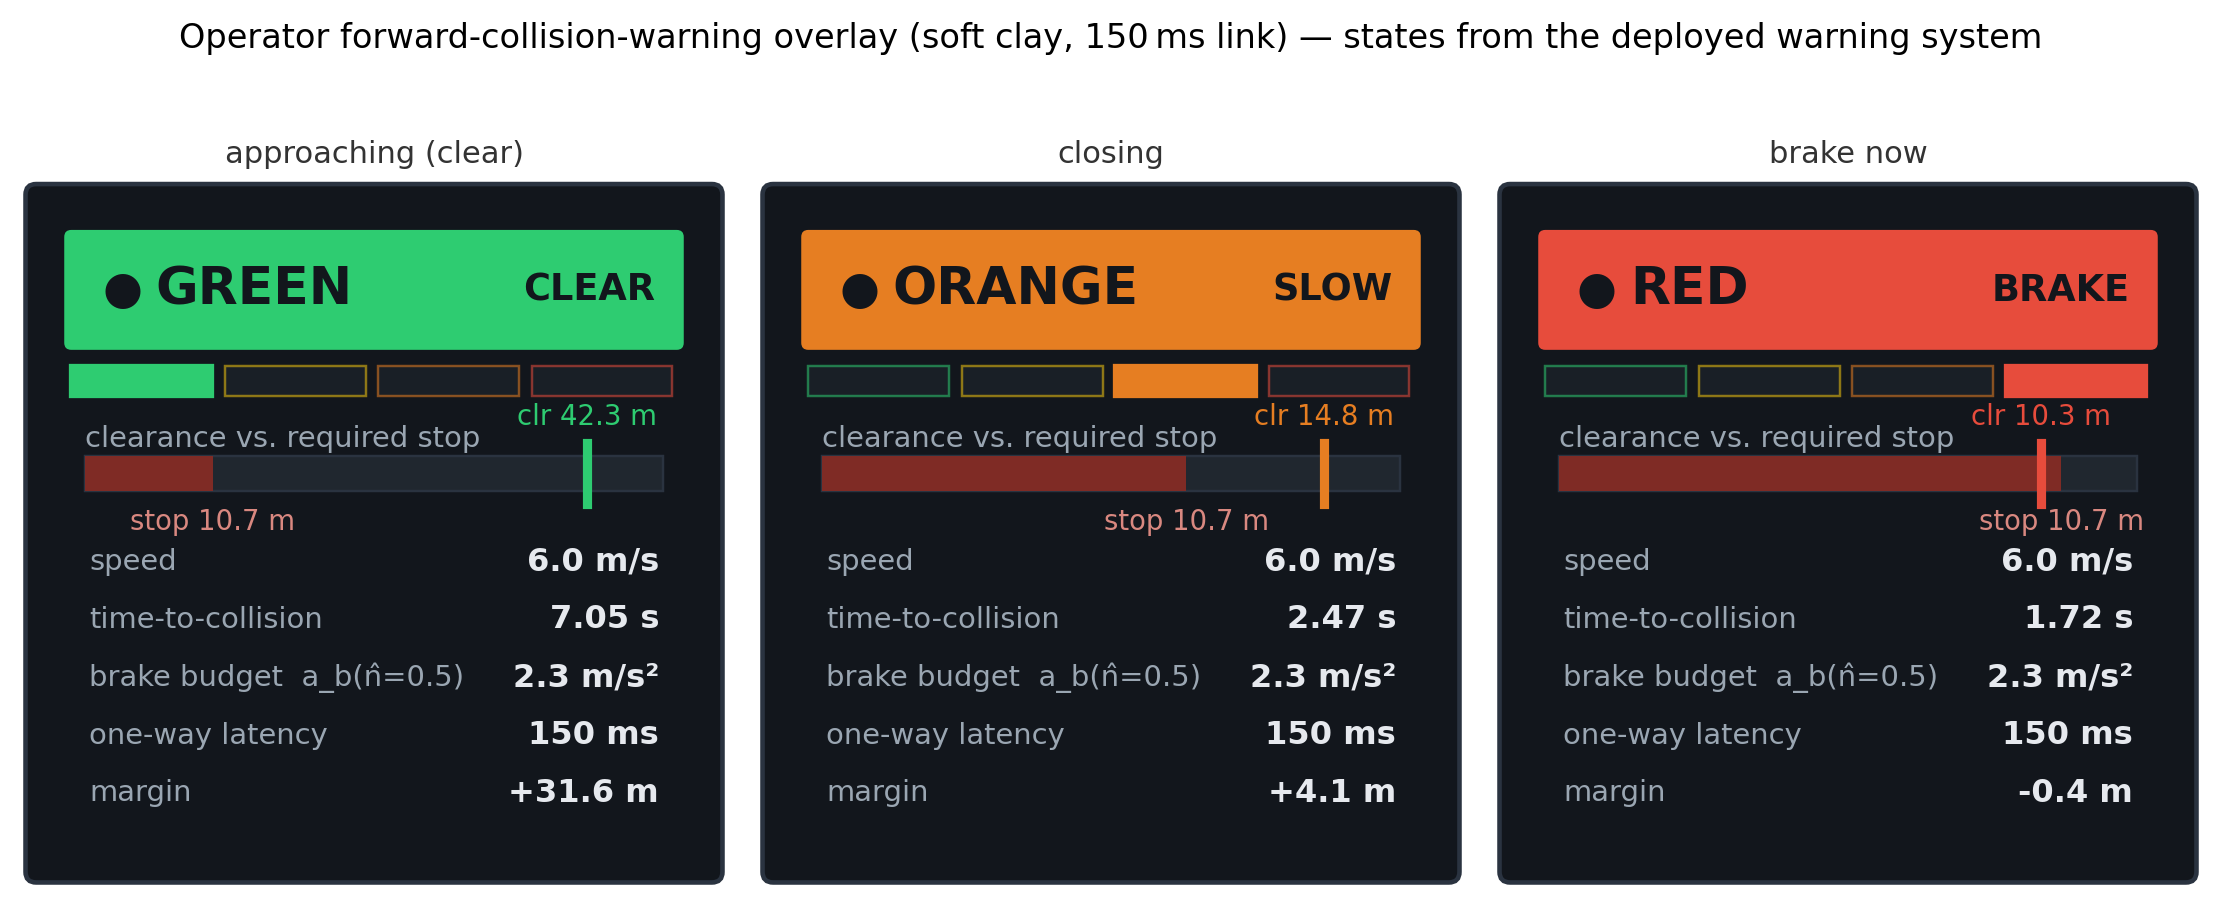
\includegraphics[width=0.98\textwidth]{warning_ui.png}
    \figcaption{Operator forward-collision-warning overlay at three moments of a
      straight-in approach (soft clay, 150~ms link), escalating
      \textsc{green}$\to$\textsc{orange}$\to$\textsc{red}. Severity, clearance
      vs.\ required stop, and the terrain brake budget $a_b(\hat n)$ are live
      outputs of the deployed warning system.}
    \label{fig:ui}
  \end{center}
\end{figure}

%------------------------------------------------------------
\section{INTEGRATED DEMONSTRATION}
As a capstone the entire stack runs on one mission (Fig.~\ref{fig:hero}): a
sinusoidal reference across a clay-to-sand soil transition through a rock field,
under the learned 5G latency, with the terrain-aware NMPC, the online Fused-UKF,
the g--g planner, the throttle observer, the DOB-CBF filter, and the collision
warning all active. The online estimate adapts across the soil boundary, the
achieved speed tracks the grip-limited reference with the observer closing the
soft-soil gap, and the safety filter keeps the traverse collision-free (closest
pass 0.99~m at the tightest rock, 140 binding-constraint avoidance steps) over
the 148~m mission. The run exercises the cross-layer interface a per-component
evaluation cannot: the estimator's live-terrain update re-conditions the safety
filter's braking authority through the same message the controller uses to
re-condition its own tire model. It is an integration check, not a separate
statistical safety claim.

\begin{figure}[t]
  \begin{center}
    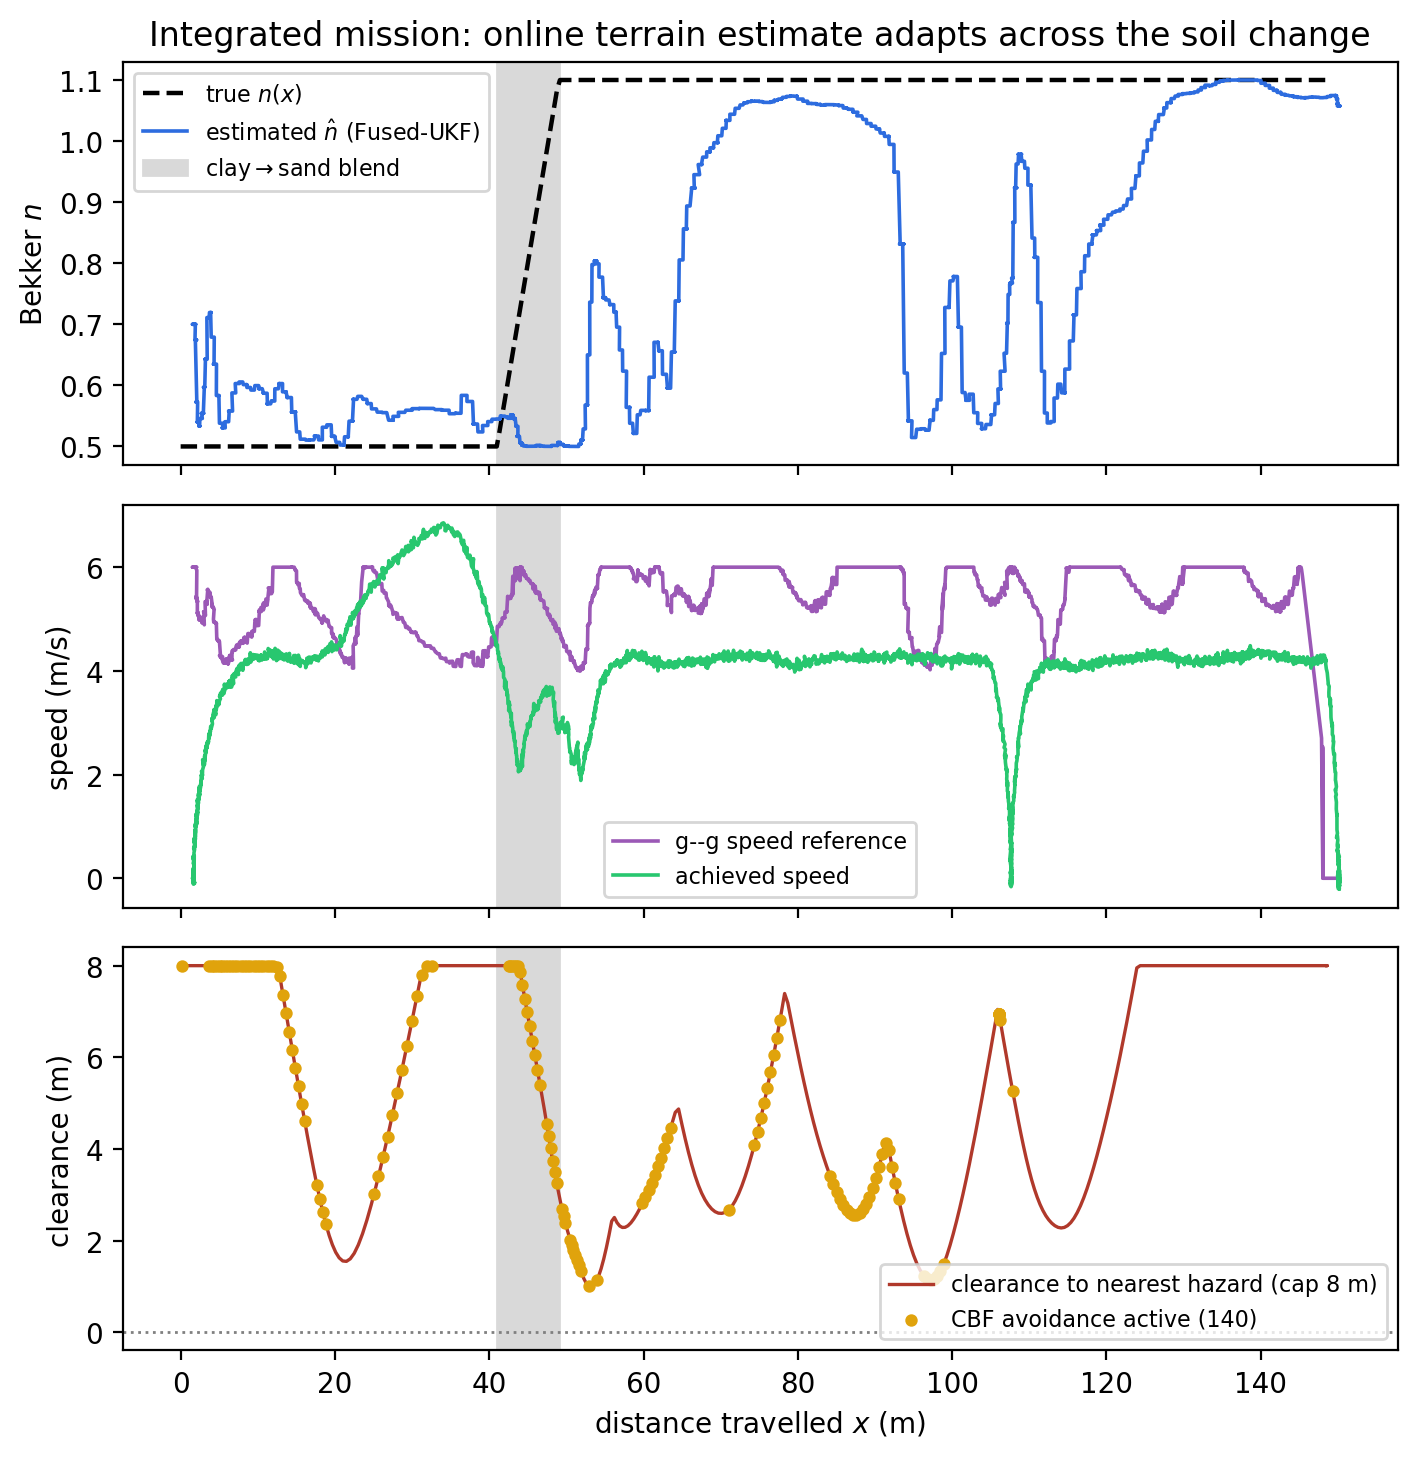
\includegraphics[width=0.92\textwidth]{integrated_hero_run.png}
    \figcaption{Integrated mission. \textbf{Top:} online terrain estimate
      $\hat n$ tracks the true $n(x)$ across the soil change (grey band).
      \textbf{Middle:} achieved speed tracks the terrain-aware g--g reference.
      \textbf{Bottom:} clearance to the nearest hazard, with DOB-CBF avoidance
      steps marked; zero collisions over the traverse.}
    \label{fig:hero}
  \end{center}
\end{figure}

%------------------------------------------------------------
\section{RELATED WORK}
Two recent threads are directly adjacent. Onozuka et al.~\cite{Onozuka25} fold
soil mechanics into a physics-informed tire structure --- a Janosi shear law
wrapped around small networks whose coefficients are re-fit online --- which is
complementary to our approach of estimating the soil and re-conditioning an
unstructured surrogate around it. Adapting their tire model into our per-axle
acados interface improved offline force prediction ($R^2_{F_y}$ from 0.35 to
0.59) but did not run stably in our in-horizon NMPC, whose static formulation
triggered solver failures on aggressive transients; since their model targets a
dedicated curvilinear-coordinate, wheelspeed-state MPC we did not reimplement,
this is a note on complementarity, not a comparison. Gupta et
al.~\cite{Gupta24} add a reinforcement-learning residual on top of MPC; on this
plant such a residual closed under 8\% of the tracking error and only at the
largest model mismatch, so we do not adopt RL compensation. Against these, the
present contribution is orthogonal: not a better tire law or residual, but the
\emph{integration} of terrain adaptation, online estimation, delay-compensated
safety, and advisory warning on one plant, where their cross-layer couplings can
be measured.

%------------------------------------------------------------
\section{CONCLUSIONS}
We presented a modular, latency-aware framework that integrates terrain-adaptive
control, online soil estimation, two-layer obstacle avoidance, and a terrain-
and latency-aware collision warning around one deformable-terrain plant. The
novelty is the integration: a differentiable SCM tire model, an online
$n$-estimator that re-conditions it, swappable safety filters, and an advisory
warning share one plant, one message stream, and one benchmarking harness, so
the main cross-layer choices are measured on comparable matrices. The
surrogate-plus-estimator recovers near-oracle tracking with no prior terrain
knowledge; the fused proprioceptive-force UKF tracks the sinkage exponent to
3.8\% median error; the DOB-CBF filter cuts collisions by 88\% under a learned
5G profile with a deterministic counterfactual attributing 36 of 45 averted
collisions to it; and the collision warning predicts stopping distance to
0.17~m. The study is entirely in simulation on Chrono's SCM and makes no
sim-to-real transfer claim; the plant is itself an extension point, so porting
to hardware or another terramechanics model is a registration rather than a
rewrite. The online estimator is scoped to the sinkage exponent, and the safety
filter is fundamentally forward-collision-avoidance; full-soil estimation, a
reachability-based filter comparison, and hardware transfer are the principal
directions for future work. An extended version reports the full ablation set,
and the benchmarking suite reproduces every non-HIL result from a single
command.

%------------------------------------------------------------ bibliography
\begin{thebibliography}{99}

\bibitem[1]{Ames19}
  Ames, A.D.; Coogan, S.; Egerstedt, M.; Notomista, G.; Sreenath, K.; Tabuada, P.:
  Control Barrier Functions: Theory and Applications.
  \newblock In Proc.\ European Control Conf.\ (ECC), pp.~3420--3431, 2019.

\bibitem[2]{Bekker69}
  Bekker, M.G.: Introduction to Terrain-Vehicle Systems.
  \newblock Ann Arbor: University of Michigan Press, 1969.

\bibitem[3]{Choi23}
  Choi, Y.-H.\ et al.: ML-based 5G Traffic Generation for Practical Simulations
  Using Open Datasets.
  \newblock IEEE Communications Magazine, Vol.~61, pp.~130--136, 2023.

\bibitem[4]{Dallas21}
  Dallas, J.\ et al.: Terrain Adaptive Trajectory Planning and Tracking on
  Deformable Terrains.
  \newblock IEEE Trans.\ Veh.\ Technol., Vol.~70, No.~11, pp.~11255--11268, 2021.

\bibitem[5]{Gupta24}
  Gupta, P.; Smereka, J.M.; Jia, Y.: Reinforcement Learning Compensated Model
  Predictive Control for Off-Road Driving on Unknown Deformable Terrain.
  \newblock arXiv:2408.09253, 2024.

\bibitem[6]{Krenn09}
  Krenn, R.; Hirzinger, G.: SCM -- A Soil Contact Model for Multibody System
  Simulations.
  \newblock In Proc.\ Int.\ Soc.\ for Terrain-Vehicle Systems (ISTVS), 2009.

\bibitem[7]{Onozuka25}
  Onozuka, Y.; Dallas, J.; Suminaka, M.; Subosits, J.: Adaptive Model Predictive
  Control on Unknown Deformable Terrains Using Physics-Informed Learning Tire
  Models.
  \newblock In Proc.\ IEEE Intelligent Vehicles Symp.\ (IV), pp.~1640--1647, 2025.

\bibitem[8]{Serban19}
  Serban, R.; Taylor, M.; Negrut, D.; Tasora, A.: Chrono::Vehicle -- Template-Based
  Ground Vehicle Modelling and Simulation.
  \newblock Int.\ J.\ Vehicle Performance, Vol.~5, No.~1, pp.~18--39, 2019.

\bibitem[9]{Shibly05}
  Shibly, H.; Iagnemma, K.; Dubowsky, S.: An Equivalent Soil Mechanics
  Formulation for Rigid Wheels in Deformable Terrain.
  \newblock J.\ Terramechanics, Vol.~42, No.~1, pp.~1--13, 2005.

\bibitem[10]{Tasora16}
  Tasora, A.\ et al.: Chrono: An Open Source Multi-Physics Dynamics Engine.
  \newblock In High Performance Computing in Science and Engineering,
  pp.~19--49, Springer, 2016.

\bibitem[11]{Zhang25}
  Zhang, H.\ et al.: Shared Control of Teleoperated Vehicles with
  Delay-Compensated Safety Filtering.
  \newblock In Proc.\ IEEE Conf.\ Control Technology and Applications (CCTA),
  pp.~192--199, 2025.

\bibitem[12]{Zhou23}
  Zhou, Z.\ et al.: A Chrono-Based Framework for Large-Scale Traffic Simulation
  with Human-in-the-Loop.
  \newblock 2023.

\end{thebibliography}

\end{document}
